
The naive algorithm for computing bisimulations in \Cref{fig:naive} is
rather inefficient as it iterates over concrete packets---a huge
space. However, in practice, the set of behaviors exhibited by a
NetKAT program is typically much smaller---it will divide the space of
packets using the Boolean classifiers encoded in forwarding tables,
and then transform the resulting partitions in a uniform way. Hence,
by encoding packets, transformations, automata, and bisimulations
using symbolic data structures, we can obtain more compact
representations and more efficient bisimulation checks. To this end,
we use a data structure called a forwarding decision diagram, which
was introduced in \cite{fastcompiler}, and is a generalization of
Binary Decision Diagrams (BDDs).

\subsection{Binary Decision Diagrams (BDDs)}

Given a set of variables $X$, a binary-decision diagram (BDD) is a
data structure that provides a compact encoding of Boolean functions
over the variables in $X$. At the level of syntax, a BDD is just a
binary tree:
\[
\BDD[X] \ni t := \top \mid \bot \mid x \mathbin{?} t \diamond t
\]
Each node in the tree is labled with a variable $x\in X$ and has two
children corresponding to the value of $x$ (and often drawn with solid
and dashed lines for the true and false cases respectively). The
leaves of the tree are $\top$ or $\bot$. Intuitively, the semantics of
a BDD follows from the fact that a valuation of the variables---i.e.,
a subset $S$ of $X$ that are true---determines a unique path from root
to a leaf. More formally, the semantics of a BDD is a function $2^X
\to 2$:
\[
\bddSem{\top}(S) = \top \qquad\qquad
\bddSem{\bot}(S) = \bot \qquad\qquad
\bddSem{x \mathbin{?} t_1 \diamond t_2}(S) = \begin{cases}
\bddSem{t_1}(S) &\text{if } x \in S\\
\bddSem{t_2}(S) &\text{if } x \not\in S
\end{cases}
\]
When working with BDDs, it is common to stipulate that it must have no
isomorphic subgraphs and that each interior node must have two
distinct children---i.e., if we try to construct a node with two
identical children, then we replace it with one of the children
instead, as the node would be redundant. Assuming the set of variables
is totally ordered, it is also common to stipulate that sequence of
variables encountered on every root to leaf path must respect the
order. BDDs satisfying these additional constraints are called
Reduced, Ordered BDDs (ROBDDs) and are canonical---i.e., a pair of
ROBDDs are equal if and only if they denote the same Boolean
function~\cite{bryant}.

\subsection{Forwarding Decision Diagrams}\label{sec:fdd}

Forwarding-decision diagrams (FDDs) generalize BDDs in three main
ways: (i) interior nodes match on packet fields rather than individual
variables; (ii) interior nodes can have mutiple children; and (iii)
leaf nodes are modeled as abstract operations from a set $M$. We
assume that $M$ that comes equipped with an interpretation function
$\val{\mathord{-}}$ into a given domain $D$. That is, for every $m\in
M$ and packet $\pk$, we have have $\val{m}(\pk) \in D$.

More formally, the syntax of \FDD s is defined as follows:
\[
\FDD[M] \ni t := m \in M \mid f \stackrel ? = \overline{\{ n\mapsto t\}} \diamond t
\]
%
The semantics of an \FDD is a function $\Pk \rightarrow D$:
\[
\fddSem{m}(\pk) = \val m (\pk) \qquad \fddSem{f \stackrel ? = \overline{\{ n\mapsto t\}} \diamond t}(\pk) = \begin{cases}
\fddSem{t_i}(\pk) &\text{if } \pk.f = n_i, \text{for some }i  \\
\fddSem{t}(\pk) & \text{if } \pk.f \not\in \{\overline{v_i}\}  \\
\end{cases}
\]
As with ROBDDs, we assume that packet fields and values are ordered,
and we order tests $f=n$ lexicographically. We also stipulate that
FDDs must have no isomorphic subgraphs and that each interior node
must have at least two unique successors. Additionally, we stipulate
that FDDs must not contain redundant tests and modifications. For
example, if the test $y=2$ is true, then $y=3$ must be false. In
addition, repeated modifications to the same header are equivalent to
just the final modification, and modifications to different fields
commute. In our implementation, we enforce the conditions for ordered,
reduced FDDs, as discussed in \Cref{sec:optimizations}.

\paragraph{Operations on FDDs.}
%
An important function on BDDs is the \emph{apply}
operation~\cite{bryant}, which combines BDDs recursively, applying a
binary operation at the leaves. It can be used to lift operations like
conjunction, disjunction, implication, etc. from Boolean values to
BDDs.  Given a function $f\colon A \to B\to C$ and two FDDs of type
$\FDD[A]$ and $\FDD[B]$, there is an analogous function that computes
a single FDD by merging the structure of the input FDDs on matching
keys and values and applying $f$ at the leaves.
\[
\binopFDD\colon (A\to B\to C)\to \FDD[A] \to \FDD[B] \to \FDD[C] \\
\]
The full definition of $\binopFDD$ is conceptually simple but
notationally tedious, so we defer it to \Cref{ap:binopfdd}.

\subsection{Symbolic \NetKAT Automata}\label{sec:sym-automata}

Recall that standard \NetKAT automata work over a huge alphabet where
there is a character for each packet. To tame this complexity we
encode the observation and continuation functions.

We first define several instantiations of \FDDs, which we will need
several additional pieces of notation.
\begin{itemize}
\item{\emph{Finite maps $X \mapsto Y$:}} defines an association between
  some set of keys $X$ and values $Y$. For example, $\{ \mathit{port}
  \mapsto 3 \}$ defines a finite map from fields to values in which
  port is associated with $3$.
\item{\emph{Symbolic packets $\FDD[2]$:}} define a set of packets.
  For example, $\top$ describes $\Pk$, $\bot$ describes $\{\}$, and
  $\mathit{dst} \stackrel ? = \{ 7 \mapsto \top \} \diamond \bot$
  describes all packets with destination address $7$. Formally, a
  symbolic packet $t$ denotes the set of packets $\pk$ for which
  $\fddSem{t}{\pk}$ equals $\top$.

  Note that we could use predicates $a \in \Pred$, complete tests
  $f_1=n_1 \cdot \cdots f_k =n_k$, or the bases found in prior
  work~\cite{coalgebraic}. We prefer the \FDD{} representation as it
  is compact and can be made canonical. We will denote symbolic
  packets as $\sympk,\sympkp, \ldots$.

  When working with symbolic packets $\sympk, \sympkp\colon \FDD[2]$,
  we will use the following infix operators corresponding to
  set-theoretic operations:
  \begin{align*}
  \sympk \cup \sympkp &= \binopFDD\ (\vee)\ (\sympk)\ (\sympkp)\\
  \sympk - \sympkp &= \binopFDD\ (\lambda a\ b\colon a\wedge \neg b)\ (\sympk)\ (\sympkp)\\
  \sympk \cap \sympkp &= \binopFDD\ (\wedge)\ (\sympk)\ (\sympkp)
  \end{align*}

\item{\emph{Symbolic updates $2^{F \Mapsto V}$:}} define
  transformations that maps an input packet to a set of
  possibly-modified packets. For example, $\{ \{\}, \{ \mathit{port}
  \mapsto 3 \}, \{ \mathit{port} \mapsto 4 \} \}$ maps any packet to a
  set containing: (i) the unmodified packet, (ii) the packet with the
  port field updated to $3$, and (iii) the packet with the port field
  updated to $4$.

  More formally, let an \emph{update} $u \in F \Mapsto V$ be a finite
  map from fields to values. We can apply an update to a packet by
  updating each field in the domain of the map to the corresponding
  value. Hence, a symbolic observation is just an \FDD with sets of
  updates at the leaves. Given an input packet, we use the \FDD to
  compute a leaf node $\{u_1,\dots,u_k\}$, create $k$ copies of the
  packet, apply the updates to each copy, and return the set of
  results.
\item{\emph{Symbolic transitions $(F \Mapsto V) \Mapsto S$:}} define
  transformations that maps an input packet to a set of
  possibly-modified packets and a successor states. For example, $\{
  \{ \mathit{port} \mapsto 3 \} \mapsto s', \{ \mathit{port} \mapsto 4
  \} \mapsto s'' \}$ maps inputs to one packet in state $s'$ with the
  port field updated to $3$ and another in state $s''$ with the port
  field updated to $4$.

  The formal semantics is similar to symbolic updates except that we
  model multicast using the outer finite map rather than a set.
\end{itemize}

A {\em symbolic} \NetKAT automaton is a tuple $(S, s_0, \epsilon,
\delta)$, where $S$ is a finite set of states, $s_0\in S$ is the
initial state and:
\begin{itemize}
    \item $\epsilon\colon S \to \FDD[2^{F\Mapsto V}]$
    \item $\delta\colon S \to \FDD[(F \Mapsto V) \Mapsto S]$
\end{itemize}

Note that our original presentation of NetKAT automata, given in
\Cref{sec:automata}, did not use a representation for packet updates,
as we formalized the types of the observation and transition functions
directly using concrete packets. The symbolic representation using
\FDD s more compactly models the behavior of the program.

\begin{figure}
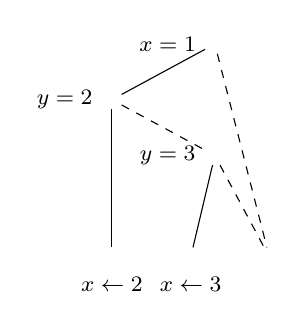
\begin{tikzpicture}[node distance=1cm] \tikzstyle{every node}=[font=\footnotesize]
\node (s0) {$\Circle $};
\node[left of=s0,node distance=0.6cm](s0l) {$x=1$};
\node[below left of=s0l](s1) {$\Circle$};
\node[below right of=s1](s2l) {$y=3$};
\node[right of=s2l, ,node distance=0.6cm](s2) {$\Circle$};
\node[below of=s1](s1p) {};
\node[below of=s1p](l3) {$\Square$};
\node[right of=l3](l2) {$\Square$};
\node[right of=l2](l1) {$\Square$};
\node[below of=l3,node distance=0.35cm](o3) {$x\gets 2$};
\node[below of=l2,node distance=0.35cm](o3) {$x\gets 3$};
\node[below of=l1,node distance=0.35cm](o3) {$\zero$};
\node[left of=s1,node distance=0.6cm](s1l) {$y=2$};
\draw (s0) edge  (s1);
\draw (s0) edge [dashed]  (l1);
\draw (s1) edge [dashed]  (s2);
\draw (s2) edge [dashed]  (l1);
\draw (s1) edge  (l3);
\draw (s2) edge  (l2);
\end{tikzpicture}\qquad\qquad
%
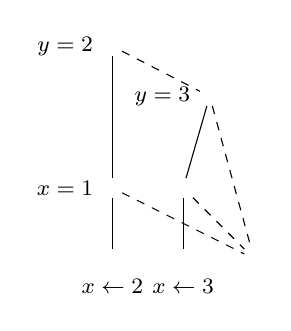
\begin{tikzpicture}[node distance=.9cm] \tikzstyle{every node}=[font=\footnotesize]
\node (s0) {$\Circle $};
\node[left of=s0,node distance=0.6cm](s0l) {$y=2$};
\node[below of=s0](s1p) {};
\node[below right of=s0](s2l) {$y=3$};
\node[right of=s2l, ,node distance=0.6cm](s2) {$\Circle$};
\node[below of=s1p](s1) {$\Circle$};
\node[right of=s1](s3) {$\Circle$};
\node[below of=s1](l3) {$\Square$};
\node[right of=l3](l2) {$\Square$};
\node[right of=l2](l1) {$\Square$};
\node[below of=l3,node distance=0.35cm](o3) {$x\gets 2$};
\node[below of=l2,node distance=0.35cm](o3) {$x\gets 3$};
\node[below of=l1,node distance=0.35cm](o3) {$\zero$};
\node[left of=s1,node distance=0.6cm](s1l) {$x=1$};
\draw (s0) edge  (s1);
\draw (s0) edge [dashed]  (s2);
\draw (s1) edge [dashed]  (l1);
\draw (s2) edge [dashed]  (l1);
\draw (s3) edge [dashed]  (l1);
\draw (s1) edge  (l3);
\draw (s3) edge  (l2);
\draw (s2) edge  (s3);
\end{tikzpicture}
\caption{Two ordered FDDs for \NetKAT program expression $x = 1;(y=2; x\gets 2 + y=3; x\gets 3)$, on the left $x \sqsubset y$ and on the right $y\sqsubset x$.}
\end{figure}

\begin{example}
The automaton from \Cref{ex:automaton} can be depicted using \FDDs as follows:

\begin{center}
\begin{tikzpicture}
  \node[rectangle, minimum size=40pt, draw, initial, label={[anchor=north, inner sep=10pt]north:$p$}] (p) {};
  \node[rectangle, minimum size=40pt, draw, right of=p, node distance=120pt, label={[anchor=north, inner sep=10pt]north:$q$}] (q) {$$};
  \node[rectangle, minimum size=40pt, draw, right of=q, node distance=120pt, label={[anchor=north, inner sep=10pt]north:$r$}] (r) {$$};
  %p
  \node[state, below left of=p, node distance=16pt, label={[distance=25pt]200:\tiny $y=2$}] (pd) {$\delta$};
  %pd
  \node[below of=pd, node distance=50pt](pd1) {$\Square$};
  \node[below of=pd1, node distance=11pt](pd1l) {\tiny $\{y\gets 7\} \mapsto q$};
  \node[left of=pd1, node distance=35pt](pd0) {$\Square$};
  \node[below of=pd0, node distance=11pt](pd0l) {$\bot$};
  \draw (pd) edge [dashed] (pd0);
  \draw (pd) edge (pd1);
  %pe
  \node[state, below right of=p, node distance=16pt, label={[distance=25pt]340:\tiny $x=1$}] (pe) {$\epsilon$};
  \node[below of=pe, node distance=50pt](pe0) {$\Square$};
  \node[below of=pe0, node distance=11pt](pe0l) {$\bot$};
  \node[right of=pe0, node distance=35pt](pe1) {$\Square$};
  \node[below of=pe1, node distance=11pt](pe1l) {$\top$};
  \draw (pe) edge [dashed] (pe0);
  \draw (pe) edge (pe1);

  %q
  \node[state, below left of=q, node distance=16pt, label={[distance=25pt]200:\tiny $z=2$}] (qd) {$\delta$};
  \node[below of=qd, node distance=50pt](qd1) {$\Square$};
  %qd
  \node[below of=qd1, node distance=11pt](qd1l) {\tiny $\{z\gets 4\} \mapsto r$};
  \node[left of=qd1, node distance=35pt](qd0) {$\Square$};
  \node[below of=qd0, node distance=11pt](qd0l) {$\bot$};
  \draw (qd) edge [dashed] (qd0);
  \draw (qd) edge (qd1);
  %qe
  \node[state, below right of=q, node distance=16pt, label={[distance=25pt]340:\tiny $z=1$}] (qe) {$\epsilon$};
  \node[below of=qe, node distance=50pt](qe0) {$\Square$};
  \node[below of=qe0, node distance=11pt](qe0l) {$\bot$};
  \node[right of=qe0, node distance=35pt](qe1) {$\Square$};
  \node[below of=qe1, node distance=11pt](qe1l) {$\{y\gets 3\}$};
  \draw (qe) edge [dashed] (qe0);
  \draw (qe) edge (qe1);

  %r
  \node[state, below left of=r, node distance=16pt, label={[distance=25pt]200:$\bot$}] (rd) {$\delta$};
  \node[state, below right of=r, node distance=16pt,
  label={[distance=25pt]340:\tiny $\{y\gets 1\}$}] (re) {$\epsilon$};
\end{tikzpicture}
\end{center}
\end{example}

\begin{remark}[Derivatives directly as \FDD s]
The derivatives presented in \Cref{fig:derivatives} can be computed
directly in terms of \FDDs. To achieve this, we simply replace $+$ and
$;$ on expressions by corresponding operations $\oplus$ and $\fatsemi$
on \FDDs.
\end{remark}

\subsection{Paths and Symbolic Analysis}

Symbolic automata based on \FDDs provide a compact representations of
a NetKAT program. However, we are not only interested in ways of
constructing automata that avoid combinatorial blowup. We also need
symbolic techniques for analyzing their transition structure. To put
it another way, we want to have operations that let us ``run'' a
symbolic automaton with symbolic rather than concrete packets.

We first define an auxiliary notion that allows us to analyze an
\FDD{}, computing the a symbolic packet that captures the set of
packets that can ``reach'' each of its leaves. We define a \emph{path}
to capture this notion.
%
\[\Paths \ni p := K \Mapsto (V \uplus \mathcal{P}(V))\]
%
Given a leaf, for each key seen on a path from the root, we either
record the value associated with the key, or the set of values that it
must not be equal to---i.e., in \FDD{} terms, the conditions needed to
take the \false branch. Note that we can represent paths in \FDD[2] as
symbolic packets.
%
\[\floor{p\in\Paths} \in \FDD[2] \]
%

Next, we can aggregate over all leaves of an \FDD{} in a path-aware
way:
\begin{align*}
    &\paths\colon \FDD[Y] \to \mathcal{P}(\Paths \times Y)
\end{align*}
The full definition of $\paths$ is given in \Cref{ap:paths}.

Now we give the method for applying a packet modification to a given
symbolic packet so that the resulting symbolic packet represents the
set of packets which could result from applying the modification to
the packets of the given symbolic packet.
%
Given a symbolic packet $\sympk\colon \FDD[2]$ and an update $u \in
K\Mapsto V$, we can define an operation
\begin{align*}
    - &\rhd - \colon \FDD[2] \to K \Mapsto V \to \FDD[2]
\end{align*}
that applies the update to the symbolic packet, yielding a new
symbolic packet. The definition is mostly straightforward, and is
given in \Cref{ap:update-op}.

With these notions fixed, we can now lift the notion of a transition
to symbolic automata and symbolic packets. Suppose we are in state $s$
of $\A$, with symbolic packet $\sympk$. Evaluating the \FDD for
$\delta(s)$, we get a map from updates to states:
%
\[ \fddSem{\delta(s)}(\sympk)\colon (K \Mapsto V) \Mapsto S \]
%
For each update in the domain of the map, we compute a new packet
(i.e., by applying the update to the symbolic packet), and a new state
$s'$, and we collect them into a set $\nextS$ of successors:
%
\begin{align*}
    &\nextS\colon S \to \FDD[2] \to  \mathcal{P}(\FDD[2] \times S)\\
    &\nextS\ (s)\ (\sympk) = \{((\sympk \cap \floor{p}) \rhd u, s') \mid (p,
    \{(u \mapsto s'), \ldots\})\in \paths\ {\delta(s)}\}\\
\end{align*}
%
We use $\nextS$ to step through through the product automaton in the
symbolic improvement in \Cref{sec:compute}.
%
The connection between standard and symbolic NetKAT automata is
captured as follows: $(\sympkp, s') \in \nextS\ (s)\ (\sympk)$ if and
only if $\sympkp = \{ \pkp \mid \delta_{\pk\pkp}(s) = s',
\pk\in\sympk\}$.

As we are analyzing symbolic automata to compute a bisimulation, it
will often be useful to step backwards. For this purpose, we define an
inverse update operator:
packet.
%
\begin{align*}
    - &\rhd^{-1} - \colon \FDD[2] \to K \Mapsto V \to \FDD[2]
\end{align*}
%
which satisfies the specification.
%
\[
    \sympkp \rhd^{-1} u = \{\pk \mid \{\pk\} \rhd u \in \sympkp\}
\]
The full definition is again in \Cref{ap:update-op}.

Analogous to the $\nextS$ function, we can define $\prevS$, which
computes the predecessors of a state in terms of symbolic packets.
%
\begin{align*}
    &\prevS\colon S \to \FDD[2] \to \mathcal{P}(\FDD[2] \times S)\\
    &\prevS\ (s)\ (\sympk) = \{(\sympk \rhd^{-1} u) \cap \floor{p}, s') \mid (p, \{(u\mapsto s'),\ldots\})\in \paths\ {\delta(s)}\}
\end{align*}
%
Conversely, we have $(\sympk, s) \in \prevS\ (s')\ (\sympkp)$ if and only if
$\sympk = \{ \pk \mid \delta_{\pk\pkp}(s) = s', \pkp\in\sympkp\}$.